%==============================================================================
\documentclass[LBMDerivation.tex]{subfiles}
\begin{document}
%==============================================================================
%
%
\chapter{推导主控方程}
%
%
%
      下一章讨论了通过使用单元体积元素d$V$来推导连续性、动量、总能量、机械(动)能、热(内)能和焓的方程式。这些方程在使用直角坐标系时被完全导出。所有讨论过的方程的摘要在 \pageref{SummationOfEquations}页给出。本章的结构(主要)如下。

%
%
\begin{itemize}
  \item 使用有限差分表达作用于体积元素。
  \item 将有限差分方程转化为偏微分方程。
  \item  操作该方程以获得保守的笛卡尔公式。
  \item 将直角坐标转换为矢量符号。
  \item 执行一个证明,以证明矢量符号的结果是笛卡尔的形式。
  \item 将方程转化为积分和非守恒形式。
\end{itemize}
%
%

	主要参考文献为
    \cite{  Bird, Versteeg, JasakPhD, Ferziger, Rappaz,  Schwarze, ProgrammersGuide}
    and \cite{Moukalled15}.
%
%
%
%
%
\section{连续性方程}
%
%
	在下一节中,将介绍连续性方程的推导。该方程本身描述了一个任意体积元素d$V$的质量平衡。

 考虑通过一个小的控制体积元件d$V$的质量流,参见图\ref{figure::massFigure},同时使用质量不转化为能量或反之亦然的约束条件,体积元件的质量平衡必须得到满足。这意味着,如果控制体积内的质量不因压缩或膨胀而改变,那么通过其表面进入和离开体积元件的质量流必须相等--这也被命名为$\textit{质量积累率}$。考虑到一个小的控制体积d$V$,我们可以说。

%
%
\begin{equation}
\left[
 \begin{matrix}
  \rmm{rate~of~mass}\\
  \rmm{accumulation}
 \end{matrix}
\right]
=
\left[
 \begin{matrix}
  \rmm{rate~of~mass}\\
  \rmm{entering~the~volume}
 \end{matrix}
\right]
-
\left[
 \begin{matrix}
  \rmm{rate~of~mass}\\
  \rmm{leaving~the~volume}
 \end{matrix}
\right].
\label{equation::massWord}
\end{equation}
%
%
	为更清楚一些,我们现在将重点放在图上\ref{figure::massFigure}。很明显,符号{\texttt{mass}}是通过速度在表面上运输的。这种传输现象被称为对流(Advection),有时也被称为平流(Convection)。在文献中,我们可以发现对流和平流的不同含义如下。
%
%
\begin{itemize}
 \item 对流(Advection): 基于流体流动(通量)的质量、动量、能量等的传输,没有扩散效应。
  \item 平流: 基于通量和扩散的任何物理量的运输。
\end{itemize}
%
%
    然而,我个人听说,对流和平流代表的总是基于通量的感兴趣的数量的运输,而对流的命名总是如果我们在谈论动量方程(例如通量的源项),而其他数量是与通量平流的。


	质量的传输发生在所有三个空间方向$x$($u_x$)、$y$($u_y$)和$z$($u_z$)。此外,质量可以在控制元素d$V$内改变,这与压缩或膨胀现象有关。因此,体积内流体的密度必须改变。

%
%
%
%
\begin{figure}[!b]
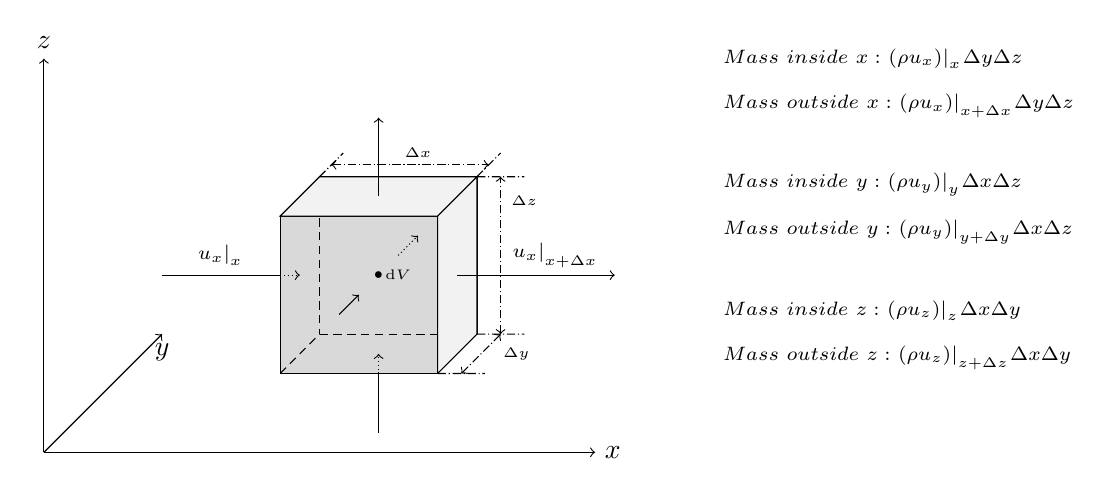
\begin{tikzpicture}
% Koordinatensystem
\draw[->] (0,0) -- (7,0) node[right] {$x$} coordinate(x axis);
\draw[->] (0,0) -- (0,5) node[above] {$z$} coordinate(z axis);
\draw[->] (0,0) -- (1.5,1.5) node[below] {$y$} coordinate(y axis);

% Quader
\draw [fill=gray!30] (3,1) -- (5,1) -- (5,3) -- (3,3) -- (3,1) ;

\draw [densely dashed] (3.5,1.5) -- (5.5,1.5);
\draw [] (5.5,1.5) -- (5.5,3.5) -- (3.5,3.5);
\draw [densely dashed] (3.5,3.5) -- (3.5,1.5);

\draw  [densely dashed] (3,1) -- (3.5,1.5);
\draw  [fill=gray!10] (5,1) -- (5.5,1.5) -- (5.5,3.5) -- (5,3) -- (5,1);
\draw  [fill=gray!10] (5,3) -- (5.5,3.5) --  (3.5,3.5) -- (3,3) -- (5,3);

%\draw (3,1) -- (3.5,3.5);
%\draw (3,3) -- (3.5,1.5);

% Pfeile
% rechts nach links
\draw [densely dotted, ->] (3,2.25) -- (3.25,2.25);
\draw [] (1.5,2.25) -- (3,2.25);
\draw [->] (5.25,2.25) -- (7.25,2.25);

% unten nach oben
\draw [] (4.25,0.25) -- (4.25,1);
\draw [densely dotted, ->] (4.25,1) -- (4.25,1.25);
\draw [->] (4.25,3.25) -- (4.25,4.25);

% vorn nach hinten
\draw [densely dotted, ->] (4.5,2.5) -- (4.75,2.75);
\draw [->] (3.75,1.75) -- (4,2);

% Punkte für Gleichungen
\node at (2.25,2.5) {\scriptsize $ u_x|_{_x}$};
\node at (6.5,2.5) {\scriptsize $ u_x|_{_{x+\Delta x}}$};

%\node at (4.5,0.5) {\scriptsize $ u_y|_{_y}$};
%\node at (4.5,4.2) {\scriptsize $ u_y|_{_{y+\Delta y}}$};

%\node at (4.5,2.75) {\scriptsize $ u_z|_{_x}$};
% \node at (4,1.75) {\scriptsize $ u_z|_{_{z+\Delta z}}$};

% Linien für dx dy dz
\draw [densely dashdotted] (5,1) -- (5.6,1)
	 (5.5,1.5) -- (6.1,1.5)
	 (5.5,3.5) -- (6.1, 3.5)
	 (3.5,3.5) -- (3.8,3.8)
	 (5.5,3.5) -- (5.8,3.8);

\draw [<->,densely dashdotted] (5.3,1) -- (5.8,1.5);
\node at (6,1.25) {\tiny $\Delta y$};

\draw [<->,densely dashdotted] (5.8,1.5) -- (5.8,3.5);
\node at (6.1,3.2) {\tiny $\Delta z$};

\draw [<->,densely dashdotted] (3.65,3.65) -- (5.65,3.65);
\node at (4.75,3.8) {\tiny $\Delta x$};

% Volumenpunkt
\node at (4.25,2.25) {\tiny $\bullet$};
\node at (4.5,2.25) {\tiny d$V$};


\node at (8.5,5) [right] {\scriptsize $ \rmm{Mass~inside~x:~} (\rho u_x)|_{_x} \Delta y \Delta z $};
\node at (8.5,4.4) [right] {\scriptsize $ \rmm{Mass~outside~x:~} (\rho u_x)|_{_{x+\Delta x}} \Delta y \Delta z $};

\node at (8.5,3.4) [right] {\scriptsize $ \rmm{Mass~inside~y:~} (\rho u_y)|_{_y} \Delta x \Delta z $};
\node at (8.5,2.8) [right] {\scriptsize $ \rmm{Mass~outside~y:~} (\rho u_y)|_{_{y+\Delta y}} \Delta x \Delta z $};

\node at (8.5,1.8) [right] {\scriptsize $ \rmm{Mass~inside~z:~} (\rho u_z)|_{_z} \Delta x \Delta y $};
\node at (8.5,1.2) [right] {\scriptsize $ \rmm{Mass~outside~z:~} (\rho u_z)|_{_{z+\Delta z}} \Delta x \Delta y $};

\end{tikzpicture}
\caption{Mass balance in a small volume element d$V$.}
\label{figure::massFigure}
\end{figure}
%
%
%
%
	更详细地分析图\ref{figure::massFigure},我们观察到速度向量与表面的法线是一致的。通过表面进入或离开体积元素的质量率被称为质量通量,它是简单的密度乘以相对于表面面积的速度。


	为了推导质量守恒方程,我们必须在控制体积d$V$的所有面上建立表面通量的平衡。换句话说,如果我们假设体积内没有质量积累(假设:不可压缩),那么里面的一切都要出去。描述表面通量的单项在图\ref{figure::massFigure}的右边给出:。

 考虑到可压缩流体,控制体积内的质量变化率d$V$与密度$\rho$有关,并且只会随着时间的推移而减少或增加。值得一提的是,这个量被定义为\textbf{每单位体积的质量}。因此,我们可以把密度的变化率写成:
%
%
\begin{equation}
 \text{Time Accumulation} = \frac{\Delta \rho}{\Delta t}~.
 \label{EQUATION::densityTime}
\end{equation}
%
%

	通过使用图\ref{figure::massFigure} 和方程(\ref{EQUATION::densityTime})中给出的数学表达式重写方程(\ref{equation::massWord}),就可以看出。

%
%
\begin{align*}
\frac{\Delta \rho}{\Delta t} \Delta x \Delta y \Delta z
&=
  \left((\rho u_x)|_{_x} - (\rho u_x)|_{_{x+\Delta x}}\right) \Delta y \Delta z \\
&+
  \left((\rho u_y)|_{_y} - (\rho u_y)|_{_{y+\Delta y}}\right) \Delta x \Delta z \\
&+
  \left((\rho u_z)|_{_z} - (\rho u_z)|_{_{z+\Delta z}}\right) \Delta x \Delta y~.
  \numberthis
\end{align*}
%
%
	用这个方程除以体积$\Delta V =\Delta x\Delta y\Delta z$,我们最终得到以下结果。
%
%
\begin{align*}
 \frac{\Delta \rho}{\Delta t}
&=
  \frac{(\rho u_x)|_{_x} - (\rho u_x)|_{_{x+\Delta x}}}{\Delta x} \\
&+
  \frac{(\rho u_y)|_{_y} - (\rho u_y)|_{_{y+\Delta y}}}{\Delta y} \\
&+
  \frac{(\rho u_z)|_{_z} - (\rho u_z)|_{_{z+\Delta z}}}{\Delta z}
  \numberthis ~.
  \label{EQUATION::ab}
\end{align*}
%
%
	引入无限小的体积元素的假设------这意味着我们减少了体积四角之间的距离,因此,$\Delta$走到极限成为零。
%
%
\begin{equation}
 \frac{\Delta}{\Delta x}
    ~ ~ \longrightarrow
    ~ ~ \lim_{\Delta x \to 0}{\frac{\Delta}{\Delta x}}
    = \frac{\partial}{\partial x}~,
 \label{EQUATION::infty}
\end{equation}
%
%
也是一个无限小的时间范围。
%
%
\begin{equation}
 \frac{\Delta}{\Delta t}
    ~ ~ \longrightarrow
    ~ ~ \lim_{\Delta t \to 0}{\frac{\Delta}{\Delta t}}
    = \frac{\partial}{\partial t} ~,
  \label{EQUATION::inftyTime}
\end{equation}
%
%
	我们可以将有限差分方程转化为偏微分方程。为此,我们必须将方程(\ref{EQUATION::infty})和(\ref{EQUATION::inftyTime})用于(\ref{EQUATION::ab})。由此可见。
%
%
\begin{equation}
 \frac{(\rho u_x)|_{_x} - (\rho u_x)|_{_{x+\Delta x}}}{\Delta x} = \frac{-\Delta (\rho u_x)}{\Delta x}
\longrightarrow
-\frac{\partial}{\partial x} (\rho u_x)~,
\end{equation}
\begin{equation}
\frac{(\rho u_y)|_{_y} - (\rho u_y)|_{_{y+\Delta y}}}{\Delta y} = \frac{-\Delta (\rho u_y)}{\Delta y}
\longrightarrow
-\frac{\partial}{\partial y} (\rho u_y) ~,
\end{equation}
\begin{equation}
\frac{(\rho u_z)|_{_z} - (\rho u_x)|_{_{z+\Delta z}}}{\Delta z} = \frac{-\Delta (\rho u_z)}{\Delta z}
\longrightarrow
-\frac{\partial}{\partial z} (\rho u_z) ~,
\end{equation}
\begin{equation}
  \frac{\Delta \rho}{\Delta t} \to \frac{\partial \rho}{\partial t} ~,
\end{equation}
%
%
%
%
	因此,一般的质量守恒(连续性)方程为:
%
%
\begin{equation}
\boxed{
 \frac{\partial \rho}{\partial t} =
 - \left(
      \frac{\partial}{\partial x} (\rho u_x)
    + \frac{\partial}{\partial y} (\rho u_y)
    + \frac{\partial}{\partial z} (\rho u_z)
   \right)
   } ~.
\end{equation}
%
%
	在使用Nabla-Operator $\nabla$和速度矢量\textbf{U}时,可以用矢量符号重写该方程。
%
%
\begin{equation}
\boxed{
 \frac{\partial \rho}{\partial t} =
 -   \nabla \bullet \left(\rho \textbf{U}\right)
   } ~.
   \label{EQUATION::massCompressible}
\end{equation}
%
%
	然而,如果我们专注于不可压缩流体,我们可以假设密度是常数,因此,量$\rho$可以从导数中取出,整个方程可以除以密度$\rho$。很明显,由于密度是一个常数,时间导数将消失。换句话说,在体积元素的时间内没有质量的积累。我们也可以用以下方式来解释它。如果我们假设密度不变,就没有膨胀或压缩现象,因此,时间导数变为零。因此,只有进入和/或离开体积元件表面的质量通量需要被考虑到。
	
  对于不可压缩的情况,流体的密度是恒定的,因此,我们可以将质量守恒方程简化为。
%
%
\begin{equation}
 \boxed{  \nabla \bullet \textbf{U} = 0} ~.
 \label{EQUATION::massIncompressible}
\end{equation}
%
%
在不可压缩的质量守恒方程的情况下,很明显,矢量符号的结果又是笛卡尔的形式。因此,这里没有演示转换的过程。如果想重新检查,只需使用方程(\ref{EQUATION::divVector})。

	\textbf{Remark}: 在许多情况下,不可压缩性意味着不存在膨胀和/或压缩现象。然而,流体密度仍然可以取决于温度,因此,这个量不是一个常数。在这种情况下,我们必须注意在计算中使用哪个质量守恒方程。要么是不可压缩的,要么是可压缩的。
	
  一般来说,如果密度不是一个常数,我们不允许使用简化的质量守恒方程(\ref{EQUATION::massIncompressible}),因为事实上,非常量不允许从导数中取出。然而,如果密度变化非常小,我们可以使用有限制的不可压缩的质量守恒方程。其原因是基于数值学和与动量守恒方程的相互作用。



%
%
\subsection{守恒定律方程的积分形式}
%
%
	为了完整起见,现在将给出质量守恒方程的积分形式。在使用高斯定理(\ref{EQUATION::gausstheorem})时,我们可以将发散项(作用于体积)转化为表面积分。元素中密度的累积是一个简单的体积积分。此外,体积元素d$V$本身并不随时间而改变其形状(固定的有限体积-静态网格)。因此,我们的结果是。
%
%

	Compressible:
%
%
\begin{equation}
 \boxed{
 \frac{\partial}{\partial t} \int \rho \mathrm{d}V=
 -   \oint \rho \textbf{U} \cdot \textbf{n} \mathrm{d}S
   } ~.
\end{equation}
%
%

	Incompressible:
%
%
\begin{equation}
 \boxed{
    \oint \textbf{U} \cdot \textbf{n} \mathrm{d}S = 0
   } ~.
\end{equation}
%
%
	表面积分的意思无非是在体积元素的表面上取得通量的平衡;什么是进去和出来。根据体积的形状,我们必须评估更多或更少的面。连续性方程的积分形式导致了所谓的有限体积法(FVM)。这种方法是保守的,我们可以将这种方法应用于任意体积,如六面体、四面体、棱镜、楔形等。这一优势使这种方法变得流行和灵活。然而,值得一提的是,体积的形状一般会影响数值稳定性和计算精度。
%
%
%
%
%
\subsubsection{\OF}
%
%
在 \OF 中,我们使用上面的方程(积分)来计算每个数值单元面上的通量。通量场被命名为\texttt{phi},通过在每个求解器中包含两个头文件中的一个来创建。
%
%
\begin{itemize}
 \item createPhi.H
 \item compressibleCreatePhi.H
\end{itemize}
%
%

	由于我们将密度和速度存储在单元中心,我们需要将这些数值内插到面中心。这个计算是通过调用函数  \texttt{interpolate(rho*U) \& mesh.Sf()}完成的。正如我们所看到的,这将简单地计算每个单元中心的密度和速度矢量的乘积,并通过包括相应的邻接单元信息将结果插值到面中心。为了得到通量,已知的面值再乘以表面法向量的大小 (\texttt{Sf()})。该计算是两个向量的内积运算,在 \OF 中用符号\texttt{\&}表示。
%
%
%
%
%
\subsection{连续性方程和物质导数}
%
%
在第一章中,在介绍基本数学运算时,我们已经提到了物质导数。在了解了连续性方程之后,我们可以更详细地研究它。

 使用物质导数公式(\ref{EQUATION::totalDerivative}),我们能够通过对发散项应用乘积规则(\ref{EQUATION::productRuleVS})重写连续性方程(\ref{EQUATION::massCompressible})。
%
%
\begin{equation}
  \nabla \bullet \left(\rho \textbf{U}\right)
=
  \textbf{U} \bullet \nabla \rho + \rho \nabla \bullet \textbf{U} ~.
\end{equation}
%
%
	将此表达式代入方程
    (\ref{EQUATION::massCompressible}), 得到:
%
%
\begin{equation}
 \frac{\partial \rho}{\partial t}
 =
 -\textbf{U} \bullet \nabla \rho - \rho \nabla \bullet \textbf{U} ~.
\end{equation}
%
%
	最终,将所有项移到LHS:
%
%
\begin{equation}
 \underbrace{\frac{\partial \rho}{\partial t}
+
 \textbf{U} \bullet \nabla \rho}_{\mathrm{Total~derivative}}
+
 \rho \nabla \bullet \textbf{U}
 =
0 ~.
\end{equation}
%
%
其结果为:
%
%
\begin{equation}
 \frac{\mathrm{D} \rho}{\mathrm{D} t}
+
 \rho \nabla \bullet \textbf{U}
 =
0 ~.
\end{equation}
%
%



%==============================================================================
\end{document}
%==============================================================================
